\documentclass{ximera}

\graphicspath{{./}{thePythagoreanTheorem/}{deMoivreSavesTheDay/}{complexNumbersFromDifferentAngles/}}

\usepackage{tikz}
\usepackage{tkz-euclide}
\usetkzobj{all}
\tikzstyle geometryDiagrams=[ultra thick,color=blue!50!black]
\newcommand{\tri}{\triangle}
\renewcommand{\l}{\ell}
\renewcommand{\P}{\mathcal{P}}
\newcommand{\R}{\mathbb{R}}
\newcommand{\Q}{\mathbb{Q}}

\newcommand{\Z}{\mathbb Z}

\renewcommand{\vec}{\mathbf}
\renewcommand{\d}{\,d}



%% Egyptian symbols

\usepackage{multido}
\newcommand{\egmil}[1]{\multido{\i=1+1}{#1}{
\includegraphics[scale=.1]{egyptian/egypt_person.pdf}\hspace{0.5mm}}}
\newcommand{\eghuntho}[1]{\multido{\i=1+1}{#1}{
\includegraphics[scale=.1]{egyptian/egypt_fish.pdf}\hspace{0.5mm}}}
\newcommand{\egtentho}[1]{\multido{\i=1+1}{#1}{
\includegraphics[scale=.1]{egyptian/egypt_finger.pdf}\hspace{0.5mm}}}
\newcommand{\egtho}[1]{\multido{\i=1+1}{#1}{
\includegraphics[scale=.1]{egyptian/egypt_lotus.pdf}\hspace{0.5mm}}}
\newcommand{\eghun}[1]{\multido{\i=1+1}{#1}{
\includegraphics[scale=.1]{egyptian/egypt_scroll.pdf}\hspace{0.5mm}}}
\newcommand{\egten}[1]{\multido{\i=1+1}{#1}{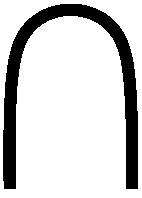
\includegraphics[scale=.1]{egyptian/egypt_heel.pdf}\hspace{0.5mm}}}
\newcommand{\egone}[1]{\multido{\i=1+1}{#1}{
\includegraphics[scale=.1]{egyptian/egypt_stroke.pdf}\hspace{0.5mm}}}
\newcommand{\egyptify}[7]{
 \multido{\i=1+1}{#1}{
\includegraphics[scale=.1]{egyptian/egypt_person.pdf}\hspace{0.5mm}}
 \multido{\i=1+1}{#2}{
\includegraphics[scale=.1]{egyptian/egypt_fish.pdf}\hspace{0.5mm}}
 \multido{\i=1+1}{#3}{
\includegraphics[scale=.1]{egyptian/egypt_finger.pdf}\hspace{0.5mm}}
 \multido{\i=1+1}{#4}{
\includegraphics[scale=.1]{egyptian/egypt_lotus.pdf}\hspace{0.5mm}}
 \multido{\i=1+1}{#5}{
\includegraphics[scale=.1]{egyptian/egypt_scroll.pdf}\hspace{0.5mm}}
 \multido{\i=1+1}{#6}{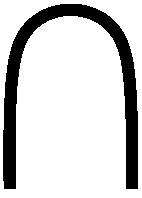
\includegraphics[scale=.1]{egyptian/egypt_heel.pdf}\hspace{0.5mm}}
 \multido{\i=1+1}{#7}{
\includegraphics[scale=.1]{egyptian/egypt_stroke.pdf}\hspace{0.5mm}}
 \hspace{.5mm}
}




\title{Limits of axioms}
\begin{document}
\begin{abstract}
In this activity, we discuss how statements can be independent of axioms.
\end{abstract}
\maketitle 

We will motivate our discussion with questions about cardinality.

\begin{question}
Given any \textit{finite} set $S$, can you prove that the power set of
$S$ has a larger cardinality?
\end{question}

Consider $S=\N$. We wish to show that $|\N|<|\P(\N)|$. Proceed as
follows: Seeking a contradiction, suppose that they are equinumerous
and imagine a bijection between every element of $\N$ and
$\P(\N)$. Call a natural number \textbf{selfish} if by your bijection
it is pared with a set containing itself. Call a natural number
\textbf{nonselfish} if it is paired with a set not containing itself.

\begin{question}
Give part of an example map between $\N$ and $\P(\N)$ and clearly
identify selfish numbers and nonselfish numbers based on your map.
\end{question}

\begin{question}
Let $B$ be the set of all nonselfish numbers. Explain why
$B\in\P(\N)$. Arrive at a contradiction. Hint: Which
integers map to $B$?
\end{question}


\begin{question}
So far we have only shown $|\N|\ne|\P(\N)|$. How do you conclude that
$|\N|<|\P(\N)|$?
\end{question}

\begin{question}
Given any set $S$, can you prove that the power set of $S$ has a
larger cardinality? Hint: repeat the argument above.
\end{question}



We know that $\N$ is countable and that $\P(\N)$ is uncountable. Define:
\begin{align*}
\beth_0 &:=|\N|\\
\beth_1 &:=|\P(\N)|\\
\beth_2 &:=|\P(\P(\N))|\\
\beth_3 &:=|\P(\P(\P(\N)))|\\
        &\vdots
\end{align*}
and so on. These are \textit{beth} numbers. From our work above we see that 
\[
\beth_0 \le \beth_1 \le \beth_2 \le \beth_3 \le \cdots
\]

\begin{question}
Let 
\[
\ph: \P(\N) \to [0,1]
\]
via the map 
\[
A \mapsto \sum_{x\in A} \frac{1}{2^x}
\]
where $A\subset \N$. Explain how every element in the image of $\ph$
can be associated to exactly one number $0.a_1a_2a_3\dots$ where $a_i=
0$ or $a_i=1$.
\end{question}

\begin{question}
Argue that $\beth_1 = \P(\N)= |[0,1]| = |\R|$.
\end{question}


On the other hand there are also \textit{aleph} numbers. Here
\[
\aleph_0 := |\N|
\]
but $\aleph_1$ is defined to be the \textit{smallest} infinite cardinal
number larger than $\aleph_0$. In general, $\aleph_n$ is the smallest
infinite cardinal number larger than $\aleph_{n-1}$. So from this
definition we find:
\[
\aleph_0 \le \aleph_1 \le \aleph_2 \le \aleph_3 \le \cdots
\]

\begin{question}
Say everything you can about the relationship between the aleph
numbers and the beth numbers.
\end{question}

\subsection*{Hilbert's first problem}


In 1900 Hilbert made a list of problems to guide the mathematicians
of the 20th Century. Here is the first problem on the list:

\begin{quote}
Prove the continuum hypothesis.
\end{quote}

What is this so-called continuum hypothesis? It states
\[
\aleph_1 = \beth_1 = |\R|.
\]

\subsection*{Hilbert's second problem}

I speculate that finding the ``holes'' in Euclid's arguments led
Hilbert to question the validity of our own proofs. This speculation
is supported by the fact that in 1900 the second problem in Hilbert's
list of problems was:
\begin{quote}
Prove that the axioms of arithmetic are consistent.
\end{quote}

\begin{question}
What would an counterexample to this claim imply? What would an
affirmative proof imply?
\end{question}

With Hilbert's second problem in mind, in 1901 Bertrand Russell showed
that the naive set theory of Cantor cannot be used to answer Hilbert's
second problem. Russell proposed that one consider the set of all sets
that do not contain themselves.

\begin{question}
How does one express this set in ``set-builder'' notation?
\end{question}

\begin{question}
 What is the problem with this set? 
\end{question}

\begin{question}
Does this set remind you of anything you've seen before?
\end{question}

The reader should rest assured that the foundations of mathematics
will not come collapsing upon our heads. Russell himself has a
resolution based on something called \textit{type theory}, though we
cannot discuss this at the moment.

\subsection*{(In)completeness}


Now we will turn our attention to Kurt G\"odel. In 1931, G\"odel
proved his (first) incompleteness theorem. To paraphrase:
\begin{quote}
Any set of axioms powerful enough to describe ``elementary number
theory'' will have statements that are \textit{true} but
\textit{unprovable}, and hence this set of axioms is incomplete.
\end{quote}

In 1940, G\"odel proved that the continuum hypothesis cannot be
disproved using the standard axioms of set theory. Around 1964, Paul
Cohen showed that the continuum hypothesis cannot be proved using the
standard axioms of set theory. To use the language of vector-spaces,
\begin{quote}
The continuum hypothesis is outside the ``span'' of our standard axioms!
\end{quote}

Hence the continuum hypothesis is one of these unprovable
statements. There are in fact, many others. Once upon a time,
mathematical statements were either true or false. Now we have a third
option, the statement could be undecidable. We have matured much since
the birth of numbers.












\end{document}
